\documentclass{article}

\usepackage{array}
\usepackage[english]{babel}
\usepackage[letterpaper,top=2cm,bottom=2cm,left=3cm,right=3cm,marginparwidth=1.75cm]{geometry}
\usepackage{amsmath}
\usepackage{graphicx}
\usepackage[colorlinks=true, allcolors=blue]{hyperref}
\graphicspath{ {resources/} }

\title{Gjallarhorn - A Kubernetes Extension}
\author{Bryan Keane}

\begin{document}

\begin{titlepage}

    \newcommand{\HRule}{\rule{\linewidth}{0.5mm}} 
    \center
    
    
    %----------------------------------------------------------------------------------------
    %	LOGO SECTION
    %----------------------------------------------------------------------------------------
    \begin{center}
        
\includegraphics{setu_logo.png}
    \end{center}
     
    %----------------------------------------------------------------------------------------
    
     
    %----------------------------------------------------------------------------------------
    %	HEADING SECTIONS
    %----------------------------------------------------------------------------------------
    \textsc{\LARGE (BSc) Applied Computing}\\[0.25cm]
    \textsc{\Large Cloud \& Networks}\\[0.25cm] 
    
    
    %----------------------------------------------------------------------------------------
    %	TITLE SECTION
    %----------------------------------------------------------------------------------------
    
    \HRule \\[0.75cm]
    { \huge \bfseries Gjallarhorn - A Kubernetes Extension}\\[0.3cm] %document
    \HRule \\[1.0cm]
     
    %----------------------------------------------------------------------------------------
    %	AUTHOR SECTION
    %----------------------------------------------------------------------------------------
    
    \begin{minipage}{0.4\textwidth}
    \begin{flushleft} \large
    \emph{Author:}\\
    Bryan Keane 
    \end{flushleft}
    \end{minipage}
    ~
    \begin{minipage}{0.4\textwidth}
    \begin{flushright} \large
    \emph{Supervisor:} \\
    Lucy White
    \end{flushright}
    \end{minipage}\\[2cm]
    
    \end{titlepage}

\newpage

\tableofcontents
\newpage

\listoffigures
\newpage

\listoftables
\newpage

\section{Plagiarism Declaration}
I declare that this material, which I now submit for assessment, is entirely my
own work and has not been taken from the work of others, save and to the extent that such
work has been cited and acknowledged within the text of my work. I understand
that plagiarism, collusion, and copying are grave and severe offences in the university and
accept the penalties that would be imposed should I engage in plagiarism, collusion or
copying. I have read and understood the Assignment Regulations. I have identified
and included the source of all other facts, ideas, opinions, and viewpoints in the
assignment references. Direct quotations from books, journal articles, internet sources,
module text, or any other source are acknowledged and the source cited are
identified in the bibliography. This assignment, or any part of it, has not been
previously submitted by me or any other person for assessment on this or any other
course of study. 


\section{Acknowledgements}
Thank people... TODO

\section{Introduction}
Atomic Kubernetes Resources is an open-source Kubernetes tool which facilitates the 
development of less problematic multi-operator containerized applications. 
Implementing this solution will allow developers to configure the custom controller 
to watch resources of their choice and connect the controller with their team’s slack 
channel to receive interactive notifications when the resource is being updated by the 
incorrect operator. Users can go as far as setting an atomic owner of resources and blocking 
other operators from making changes.

\subsection{Background}
In 2022 I completed an 8-month internship at Red Hat for my 3rd-year work placement. I worked on 
the Red Hat OpenShift API Management (RHOAM) team. RHOAM utilises multiple OpenShift Operators 
(automatically managed and configured applications) to provide a comprehensive API solution to its 
customers. The API management features provided include
\begin{itemize}
    \itemsep0em 
    \item Limiting the number of API requests based on the customer’s purchased quota
    \item Creating security policies to manage API access
    \item Monitoring API health
    \item An API portal for sign-up and documentation
\end{itemize}

While working on this team, I had the opportunity to contribute to applications which utilize 
various technologies like Kubernetes, OpenShift, and Go Operators.

\subsection{Motivation}
I encountered various problems during my internship. One of which was with RHOAM’s rate-limiting 
service and is the motivation for Gjallarhorn. Rate-limiting is done with the Marin3r Operator for 
OpenShift clusters (Red Hat’s container orchestration platform). It works by injecting a rate-limiting 
container into the Pod being rate-limited. The container works by acting as a middleman for requests. 
It  takes in requests and sends them to the destination container if the rate of requests has 
not reached the limit. The bug I found was that the port to send requests through the rate-limit 
container was being overwritten by a rogue Operator and set back by the owner Operator. This 
meant that customers who had RHOAM installed were not being consistently rate-limited. As a 
result, an influx of requests could have overloaded Pod CPU and Memory, causing needless stress 
to the cluster. It took multiple days of debugging to figure out what was going wrong and another 
week passed before my code changes were merged. This meant that this problem had been occurring on 
customer clusters for an unknown amount of time before the fix reached customers. After speaking to 
developers on various Red Hat teams, it became apparent that this problem was not unique to our team 
and is an issue that all Kubernetes and OpenShift product teams face. Fixing this will not only 
benefit Red Hat teams but any team working on a Kubernetes-based application.

\subsection{Problem Statement}
In Kubernetes (K8s), custom resources consist of YAML files which store the desired state of 
an object (a resource in Kubernetes like Pods and Deployments). An Operator can become a watcher 
(observer and/or editor of a resource's state) of an object, where it will compare the current state 
of that object with the desired state stored in its YAML file. If the states differ, the 
operator’s controller will reconcile the object’s state so that they match. This is an integral 
part of how Kubernetes functions, but it has its flaws. 

\begin{figure}[!hb]
    \centering
    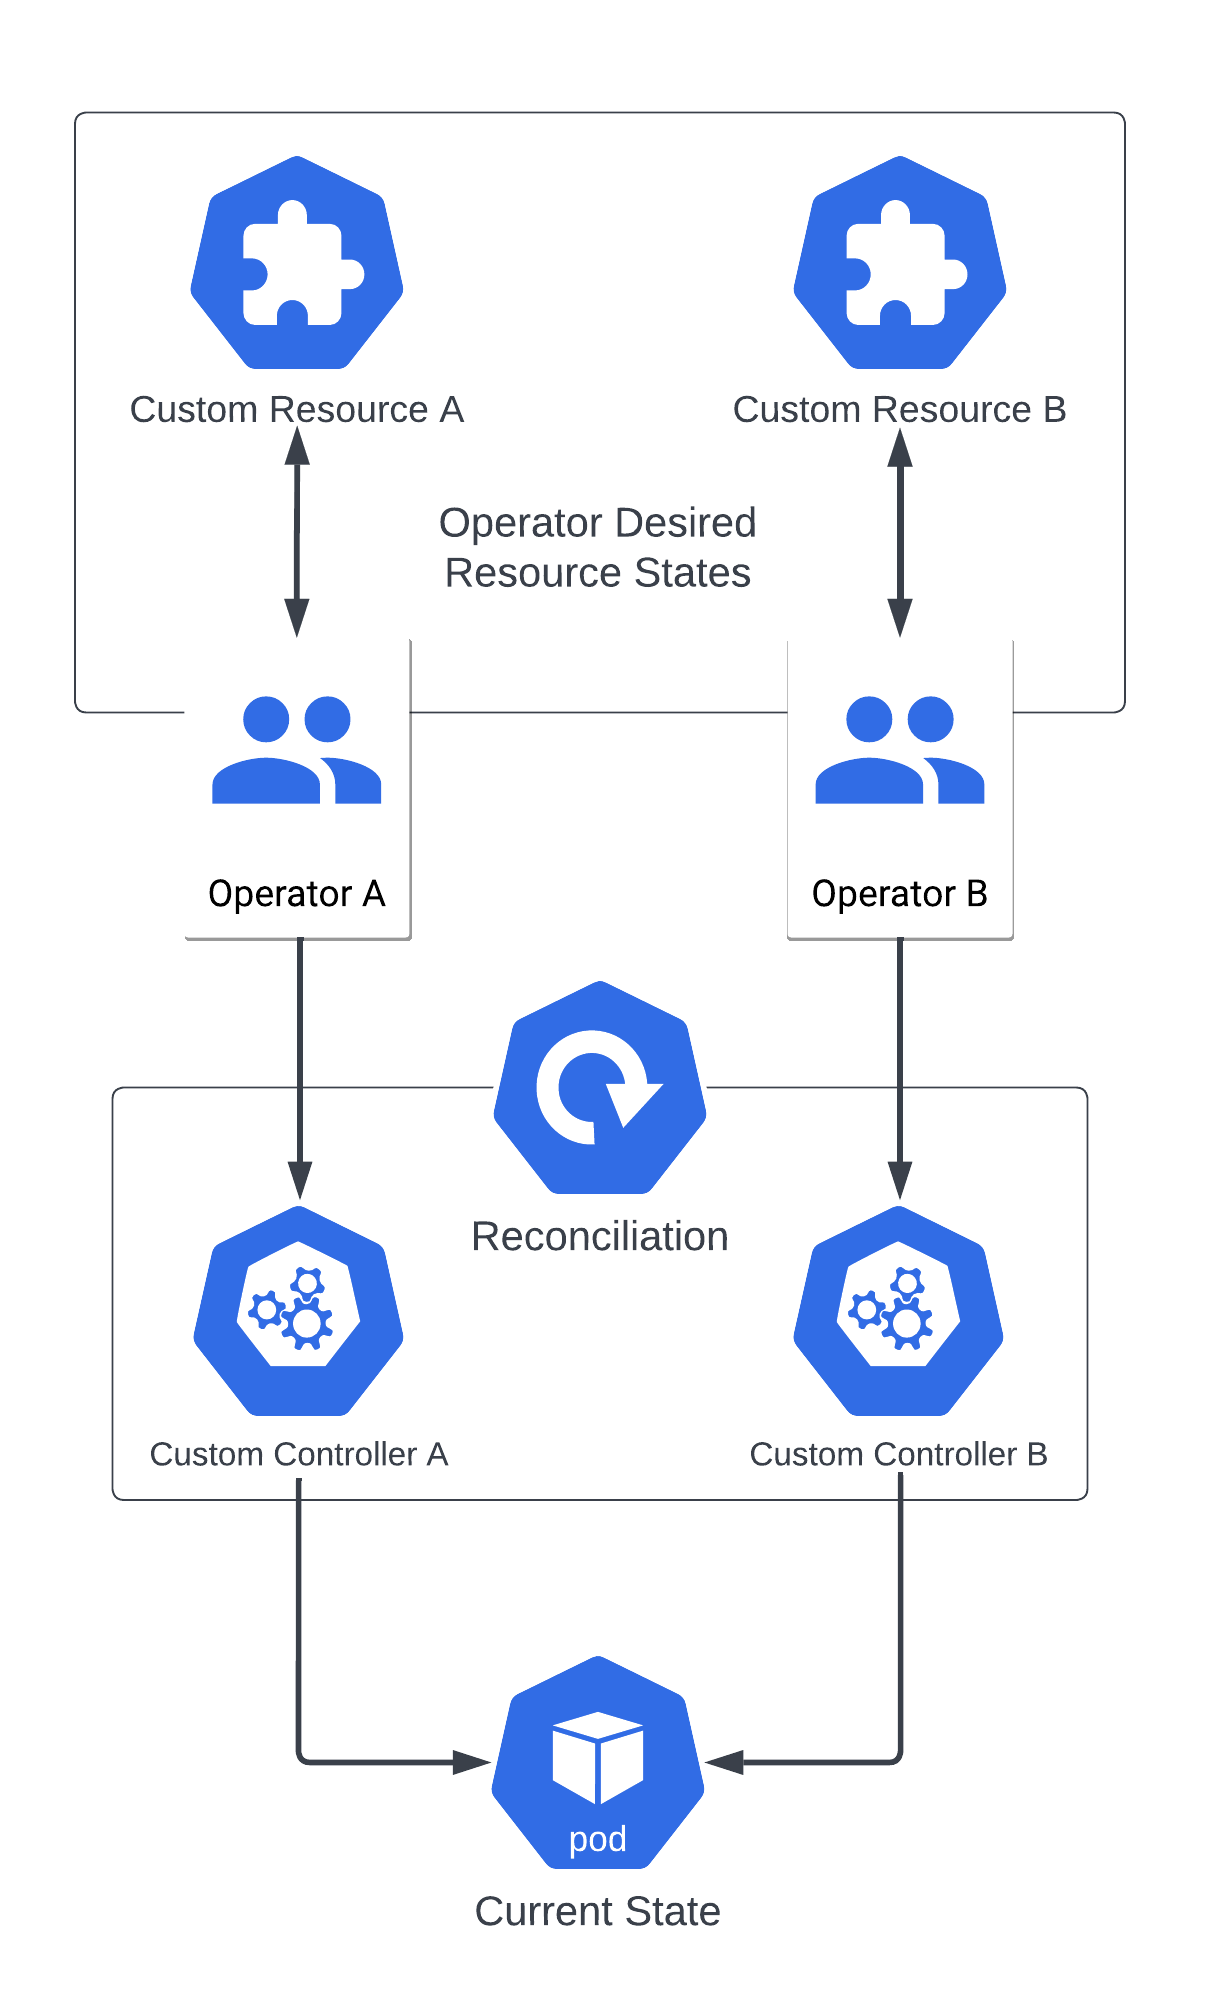
\includegraphics[width=100mm]{problem-model.png}
    \caption{Model of a common problem in multi-operator Kubernetes clusters}
    \label{problem-model}
\end{figure}

Kubernetes natively supports multiple operators to watch the state of a single resource. This can 
cause problems like the one described in Figure \ref{problem-model}. This can cause issues 
with object states and is the foundation of this project. During my Internship, I was working 
on a ticket which involved implementing pod count auto-scaling where the number of pods scales 
up based on the amount of load each pod is experiencing. During this work, I observed some 
peculiar behaviour. When I forced the pod’s load to increase the number of pods increased as 
expected, but shortly after the pod count returned to its original number. After observing for 
some time, it became apparent that something was scaling the pods up and down continuously. 
I discovered it was two OpenShift Operators fighting over the state of the pod. Each operator 
had a desired state for the pod’s deployment, where one operator wanted three replicas of the 
pod and the other operator wanted two replicas so they underwent a sort of tug-of-war, fighting 
over how many pods should be running. This is a common problem where two operators can watch 
the same resource and have conflicting resource definitions, so the operators' controllers 
fight to keep the pod in their preferred state. It is a waste of resources and can cause interruptions 
for the end user.

\subsection{Industry Example}
TODO: Split up the Problem statement into how the problem works exactly and an example in a 
context different to the one I encountered

\subsection{Aims and Objectives}
The solution is to create a custom Kubernetes controller which will monitor resource states. 
A Kubernetes Operator can create a resource, become its owner, and will set the controller to 
watch that resource for changes. If the resource is changed by another operator the controller 
will fire an alert, notify the developer via a slack integration and allow the developer to 
fix the problem without the need for time-consuming debugging. 

\begin{figure}[!hb]
    \centering
    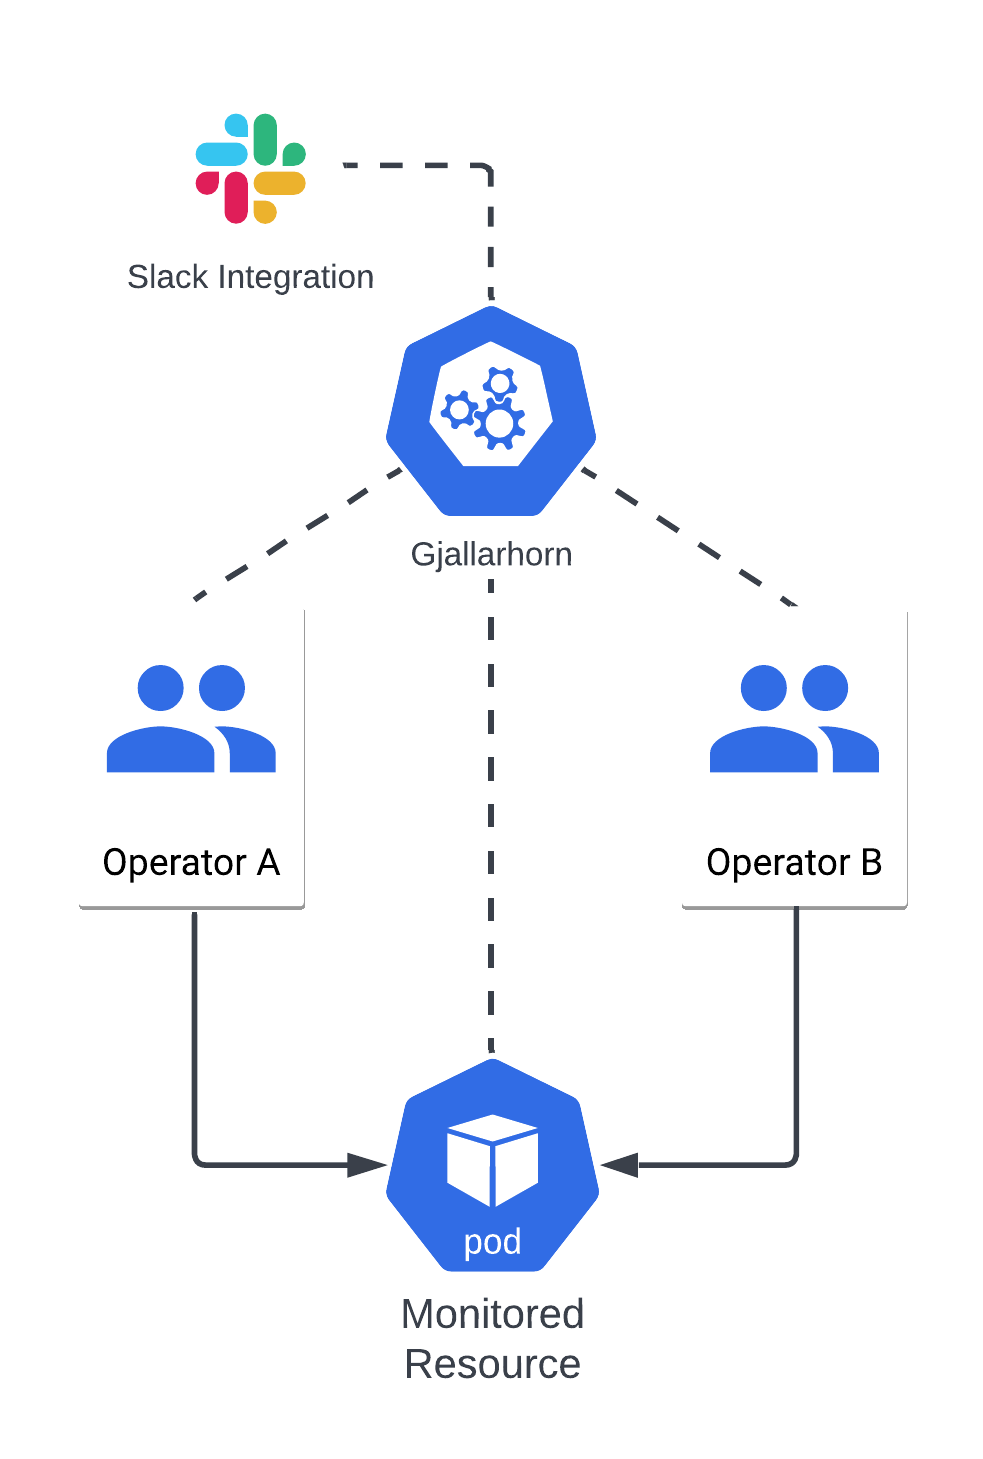
\includegraphics[width=75mm]{solution-model.png}
    \caption{Model of the solution: Gjallarhorn}
    \label{solution-model}
\end{figure}

Figure \ref{solution-model} models the proposed solution where Operator A represents the owner 
operator of the Monitored Resource, and Operator B represents the rogue operator which is 
causing the resource to change from the owner’s desired state. Once Operator A is installed, 
it creates the resource and instructs Gjallarhorn to monitor the resource’s state. Once Operator 
B is installed and changes the resource. Gjallarhorn sees this occurring and will send the 
developers a notification through slack which will remove the need for debugging and allow 
the developer to get a fix pushed as soon as possible. The stretch goal for this product 
would be to completely block Operator B from changing the resource so the developers have an 
interim solution to the bug while they push a fix to the relevant operator, preventing any 
customer downtime.

\subsection{Risks}
TODO(): this is a risky project as it has never been done before 

\subsection{Contributions}



\subsection{Outline}



\section{Methodology}
The chosen methodology for software development teams is paramount for successful planning
and development of a product. Currently the most common methodology used is Agile, but before
this the Waterfall Methodology was the gold standard. This method of development involves a distinct
sequence of actions for engineers to follow. In short, it involved extensive design and planning
before ever writing a line of code. Long documents detailing product design and strategy were 
written to fit the stakeholder's requirements. This proved to be ineffective as for most cases,
holes in the design are discovered after beginning the implementation. In recent years, Agile has
began replacing this framework as it has proven much more efficient for software development teams.



\subsection{Agile}
"Agile is an iterative approach to project management and software development that helps teams
deliver value to their customers faster and with fewer headaches" \cite{what-is-agile}. TODO()


DISCUSS AGILE + SCRUM

\subsection{Scrum Roles}
Scrum has three main roles: Scrum Master, the Product Owner, and the Development Team. These are
used to help describe the responsibilities of each stakeholder for a product. In the case of Gjallarhorn,
I will act as all of these roles as the sole developer of the project.


\subsection{Scrum Artifacts}
Teams who practice Agile and Scrum methodologies often collect Scrum Artifacts. These 
are pieces of information that a product's stakeholders and the team developing it use to 
describe its development. The main Scrum Artifacts used for this project include Product Backlog
Refinement, Sprint Planning, and Sprint Reviews. There are also various Extended Artifacts
that are not included in the official Scrum Artifacts definition. These include reporting mechanisms like
Burndown Charts.


\subsection{Version Control}
What is VCS, Git, GitHub, 


\subsection{Continuous Integration}
Version control lies at the heart of Continuous Integration. CI is an Agile practice of 
integrating code changes to a product automatically from various contributors (product 
teams and open-source community contributions). It is a method used to consistently merge 
code changes into one central repository which runs automated tests and builds to ensure 
code functionality and integrity.   



\subsection{Continuous Delivery}
Continuous Delivery is an approach 


\subsection{Testing Approach}



\subsection{Open Source}



\section{Technologies}
Kubernetes, Golang, 


\section{Tools}
Minikube, Kubebuilder, Docker, Podman, Git, GitHub, Jira


\section{Design}



\subsection{System Architecture Overview}



\subsection{Requirements}



\subsection{Functional Requirements}



\subsection{Non Functional Requirements}



\subsection{Core Requirements and Stretch Goals}



\subsection{User Stories}
As a Developer, I want to be aware of changes to resources that I own.
In order to be aware of changes to resources that I own, as a k8s developer, I want to be notified by some channel, such that I don’t have to manually watch resources in a cluster.
As a Developer, I want to control the cadence of alerts so that I can control noise created from alerts.
As a Developer, I want to claim ownership of the resources that I control
As a Developer, I want to control the changes to resources that I own.


\subsection{Personal Stories}
As a student, I want to have achieved a First Class Honors, so that I can reach my academic goals
As an aspiring Software Engineer, I want to have contributed a solution to a common problem faced by Software Engineers working with Kubernetes, so that I can make a valuable contribution..?? - something like that



\subsection{User Definitions}



\subsection{Models}



\section{Prototype}



\subsection{Proof of Concept}



\section{Reflection}



\section{Summary}



\subsection{Review}



\subsection{Semester 2 Outline}



\section{Appendices}


\bibliographystyle{alpha}


\clearpage
\begin{thebibliography}{9}


\bibitem[What is Agile?, 2022]{what-is-agile}(accessed Oct. 24, 2022). 
\emph{Atlassian}, \\URL: https://www.atlassian.com/agile 



\end{thebibliography}




\end{document}